%!TEX root = ../abgabe.tex

\section{Gestaltungsregeln und Hinweise}

Geschrieben von: Saulius A

In diesen Kapitel werden verschiedene Gestaltungsprinzipien vorgestellt, die bei einer Gestaltung und Entwicklung von Applikationen und Webseiten (später meist nur Applikationen) für einem mobilen Kontext zu beachten sei. Viele der vorgestellten Prinzipien sind nützlich für eine breite Palette von Geräten, die in mobilen Kontext benutzt werden können. Es wird aber vorwiegend auf die auf die Gestaltung von der Applikationen für die Smartphones in Betracht gezogen. Am Ende dieses Kapitels, werden Gestaltungshinweise für die Entwicklung der Applikationen in Wearable Computing kontekt vorgestellt, die auch spezielle Anforderungen erfühllen müssen.

Seit der stetige Verbreitung von Smartphones und mobilen Geräten in alltäglichen Leben, steigt auch die Benutzung von Applikationen in mobilen Kontexten. Dabei stoßen viele der Benutzer, die auf ihren mobilen Gerät auf vorhandene Dienste zugreifen wollen meistens auf viele Usability Probleme. Solche Probleme liegen nicht nur in Inhaltsstruktur oder Visuelle Kommunikation, sondern auch in der Funktionen, die Dienste anbieten. Es liegt daran, dass die vorhandennen Diensten für die Erledigung von Aufgaben auf einem stationären Rechner gestaltet wurden. Dabei beachten die Dienste nicht die Einschränkungen sowie Vorteile, die der mobiler Kontext und Geräten für den Benutzer bedeuten.

Bei schon vorhandenen Applikationen muss meistens nur der Design von, sondern auch die Funktionalität der Applikationen an den Geräten, die Benutzungsumgebung und Benutzer Intentionen angepasst werden. Jakob Nielsen erwähnt in seinem Artikel \footnote{http://www.nngroup.com/articles/mobile-site-vs-full-site/, es ist ein Ausschnitt aus Bericht "Mobile Website and Application" http://www.nngroup.com/reports/mobile-website-and-application-usability/} die Hauptideen, für die Optimierung der Vorhandenen Webseiten für mobile Nutzung helfen sollte:
\begin{itemize}
	\item \textbf{Beschneide Funktionalitäten}. So sollen nur Funktionen angeboten werden, die Anwendungsfallen in  mobilen Kontext passen
	\item \textbf{Beschneide Inhalt}, um die fülle von Text zu verkleinern und um die sekundäre Informationen in anderen Seiten zu verlagern
	\item \textbf{Vergrößere Elemente der Benutzeroberfläche}
\end{itemize}

Es wird viel darüber gestritten, ob es die Ideen von Jakob Nielsen einen Richtiger Weg für die Entwicklung von Applikationen für mobilen Geräten zeigt\footnote{http://www.netmagazine.com/opinions/nielsen-wrong-mobile}. So wird es vorgeworfen, etwa dass man statt nur Beschneidung der Funktionalitäten auch auf die Zusatzmöglichkeiten der mobilen Geräten berücksichtigen sollte. Die Möglichkeiten der Informationsaufbereitung werden in Kapitel \ref{sec:Informationsaufbereitung} vorgestellt, und sollte bei der Erstellung von Applikationen erwogen werden. Als weiteres werden die Anforderungen an den Bedienelementen sowie die Interaktion in Kapitel \ref{sub:Benutzerschnittstellen}vorgestellt. Da auch Dienste bestimmte Anforderungen erfühlen sollten, werden diese in Kapitel \ref{sub:gestaltung_von_diensten}vorgestellt.

In diesen Kapitel werden keine generelle Gestaltunsprinzipien vorgestellt, sondern nur auf die Konzentriert, die für den mobilen Geräten sowie mobilen Kontext als wichtig erschienen.

\subsection{Bedienelementen und Interaktion}
\label{sub:Benutzerschnittstellen}

Es gibt eine Vielzahl von Smartphones, sowie deren Benutzerschnittstellen. Der Benutzer kann die mit einem Gerät entweder über einem Touchscreen, Tastatur, Zifferblock, Trackpoint usw. Interagieren. Jeder diese Eingabegarten hat einen anderen Charakter, daher werden die Regeln mehr für Eingabe mittels Touchscreen berichtet.

HIER NOCH TEXT

\subparagraph{Bedienelementen auf der graphische Oberfläche} 
\label{subp:gro_ere_interface_elementen}

Die Einschränkungen durch einen kleinen Bildschirm auf einen Smartphonen mussen bei der Erstellung von GUI besonders beachtet werden. So muss die Physischen Eigenschaften des Fingers  bei der Erstellung von Elementen, die mit einem Finger bedient werden beachtet. Laut einer Stunde von MIT Touch Lab, ist der Menschliche Finger im Durchschnitt etwa 10-14mm breit, und die Fingerspitze etwa 8-10 mm\cite{Srinivasan:2003uu}. In der Studie von Pekka Parhi et.al \cite{Parhi:2006gh} wurde erforscht welche optimale große von Bedienungselementen für eine Ein-handige Daumeninteraktion ist. So wurde erfahren, dass es keine signifikanten Unterschiede in der Bedienung von Elementen bei einer Elementengroße ab $>$ 9,5 \textit{mm} bei getrennte, sowie $>$ 7.7 \textit{mm} bei seriellen Erledigungen der Aufgabe existieren. Auch die Hersteller von mobilen Betriebsystemen schlagen änliche maße für Bedienelementen vor. Apple setzt eine Mindestgröße von 44 x 44 Punkten \cite{Apple}, Microsoft 7 \textit{mm} oder 26 \textit{px}\cite{lukeGUI} für Elementen voraus.

Nich nur die große der Elemente, sondern auch der Zwischenabstand zwischen diese wichtig für eine benutzerfreundliche Bedienung der Anwendung. Wie man schon in Bild (HIER FOTO mobilefirst 79) zu sehen ist, muss hier der Benutzer sich anstrengen, um den Richtigen Element in der Liste auszuwählen. Auch die unbeabsichtiges Anklicken von "Cancel" Bedienelemnt kann in Beispiel (cacel) erfolgen. So ist es empfohlen einen Abstand, sogenanten Whitespace, zwischen Bedienenlemnten zu benutzen. Solche Abstände sollten midestens von 2\textit{mm} oder 8\textit{px} betragen\cite{lukeGUI} um die unbeabsichtige Einhaben zu vermeiden.

\subparagraph{Anordnung von Elementen} 
\label{subp:anordnung_von_elementen}

Eine richtige Auslegung von Elementen in der Benutzeroberfläche, kann den Benutzer helfen ohne Kraftaufwand oder Wechsel von der Haltung des Geräts auf die wichtigen Funktionen zuzugreifen. Eine Einhändige interaktion mit den Smartphone sollte ermöglicht werden, um den Bedienen der Applikation in mobilen Kontext zu erleichtern. So wird emphohlen die wichtigen Elemente so auszulegen, dass sie leicht mit den Daumenfinger erreicht werden \cite[Seite 209]{mobileFrontier}. Da es etwa 70 bis 90 $\%$ der Menschen Rechtshändig sind, ist es laut \cite[Seite 72]{mobileFirst} verbreitet die Elementen  nach der Bequemlichkeit für den Daumenbewegung in 3 Bereichen auszulegen, wie im Bild~\ref{fig:rechtsPositioning} zu sehen sind. Da es aber keine Benutzer benachteiligt werden sollten und anhand der Ergebnisse aus der Studie \cite{Park:2010tu} können die Bereiche so aussehen, wie im Bild~\ref{fig:forallPositioning}\cite[Seite 72]{mobileFirst}.

Die Bedienungselementen, die sehr oft in der Interaktion benutzt werden, sollten in Bereicht "Leicht" platziert werden, da sie leicht mit den Daumen erreicht werden können. Die Elemente in "Ok" bereicht, brauchen schon ein wenig mehr Daumenbewegung bieten weniger Komfort. In Bereichen "Greifen" können elemente für Navigation angeboten werden, und dieses Breich benutzen von "Greifen"-Bewegung für den Daumen bedeutet.

\begin{figure}
	\centering
	\begin{subfigure}[b]{0.3\textwidth}
		\centering
			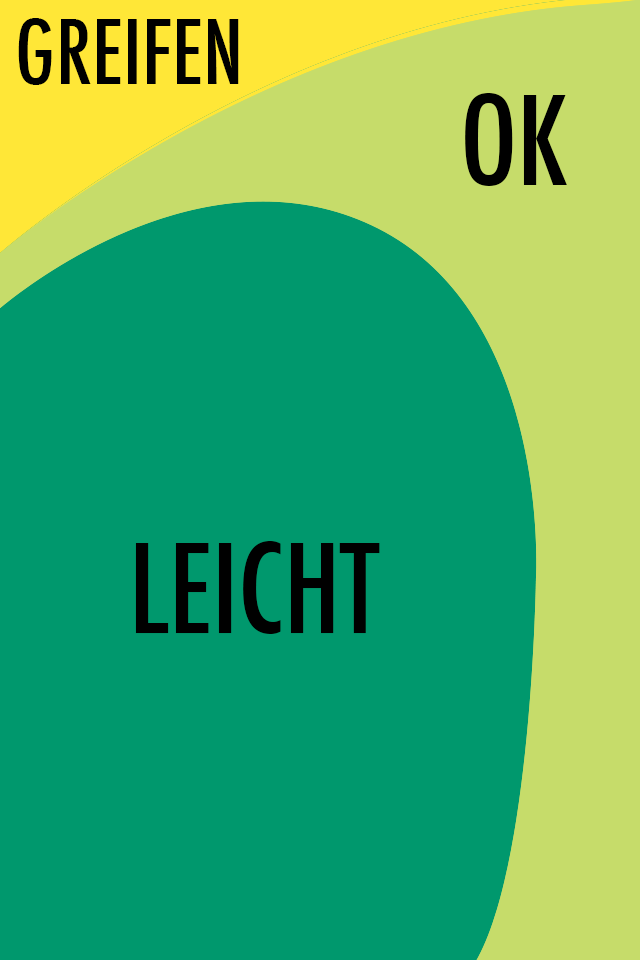
\includegraphics[width=1\textwidth]{img/anordungDerElementeSimple.png}
			\caption{Für Rechtshänder\linebreak}\label{fig:rechtsPositioning}
	\end{subfigure}
	\begin{subfigure}[b]{0.3\textwidth}
		\centering
			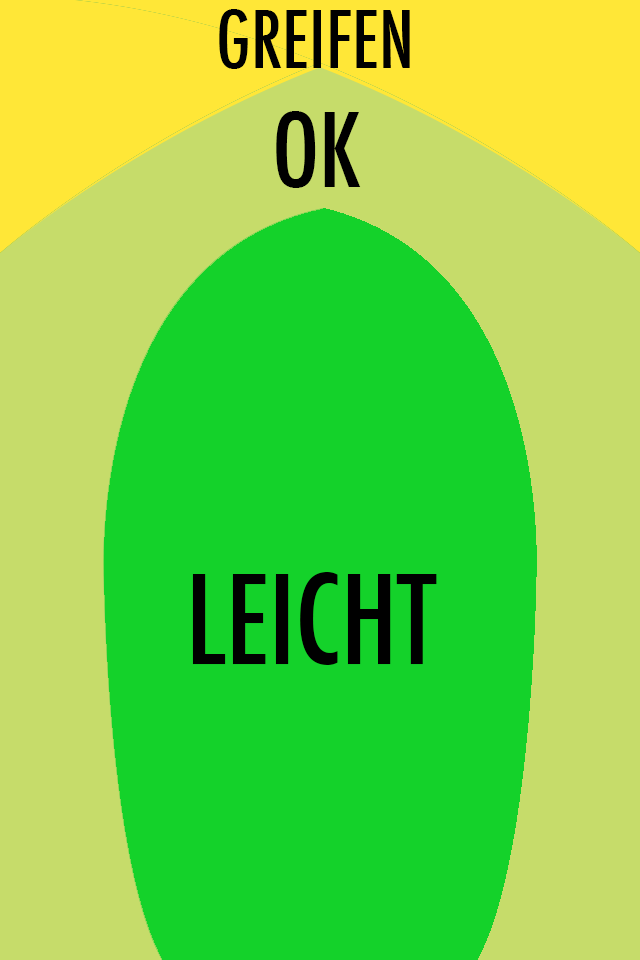
\includegraphics[width=1\textwidth]{img/anordungDerElementeForAll.png}
			\caption{Für Links- und Rechthänder, angepasst anhand Studie \cite{Park:2010tu}}\label{fig:forallPositioning}
			
	\end{subfigure}
	\caption{Positionierung von Elementen}\label{fig:elementPos}
\end{figure}


\subparagraph{Vorsicht bei NUI} 
\label{subp:benutze_nui}

Die meisten Touchgeräten bieten eine direkte Eingabe, mit denen Naturelle Gesten möglich sind. Dabei läuft man in der Gefahr, den Benutzer die Bedienbarkeit zu erschweren anstatt zu erleichtern. In mobilen Kontexten können viele situationen auftreten, in den man nur eine Hand bzw ein Finger für den Bedienung des Smartphones benutzen kann. Dadurch werden Gesten, für deren Ausführung mehr als ein Finger nötig ist, nicht nutzbar. So solte man über alternative Möglichkeiten zur Ausführung solcher Interaktionen nachdenken. Wie in Beispiel im Bild~\ref{fig:nuibsp} bietet die vorgeschlagene Benutzeroberfläche\footnote{Ausschnitt aus OpenSteetMap.com} alternative für die Pinch oder Spread Gesten einen Schaltknopf. Beim Drücken dieses Schaltknopfes, kann die karte verkleinert oder vergrößert. 

\begin{wrapfigure}{r}{0.5\textwidth}
	\begin{center}
	
	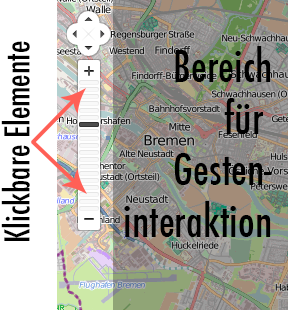
\includegraphics[width=0.3\textwidth]{img/NUIbsp.png}
	\caption{Alternative Interaktionsmöglichkeiten}\label{fig:nuibsp}
\end{center}
\end{wrapfigure}

\subparagraph{Designe für Wechselde Umgebungen} % (fold)
\label{subp:designe_f_r_au_eneinsatz}

Bei Bewegungen, ändert sich die Umgebungen. Und die Umgebungen haben verscheide Eigenschaften. So kann zum Beispiel ein Benutzer der aus ein Helligen Tag ins dunkelen Kinosaal geht, und dabei versucht weiter sein Smartphone zu benutzer, einfach überblendet von der starke leuchkraft des Bildschirms. So ist es auch empfehlenswert, Bedienelemente leicht erreichbar zu platzieren, um die Helligkeit ( vgl. \cite[ff Seite 418]{mobileInteraces}) zu regulieren oder die Farben der Benutzeroberflächen zu invertieren

\subsection{Informationsaufbereitung}
\label{sec:Informationsaufbereitung}

% - Funktionalität für mobilen kontext, seite 57 mobileFirst. In buch tapwothy sind 3 mobile behavour: micro-tasking, im local, am bored. Google teilt menschen ins urgent now, repetitve now, bored now

Menschen in mobilen Kontexten haben viele Anforderungen an der Applikationen die anders sind als für stationären Arbeitsplatzen. Um gut benutzbare Software für solchen Szenerien zu entwickeln, ist daher wichtig die Aktionen sowie Verlangen von Benutzer zu wissen und zu berücksichtigen. Man sollte wissen, wieso und wann benutzen die Anwender den Smartphone in mobilen Kontext. Eine Einteilung von Benutzer kann dabei helfen, spiezielle wünsche, sowie erwartungen an der Applikationen herauszufinden.

Die Einteilung, kann laut Google anhand derens Verhaltens einggeteilt werden. So wurden drei Grupen indentifiziert: "urgent now", "repetitive now", "bored now"\cite{googleUsers}. Benutzer der Gruppe "Urgent now" wollen ein wenig Infomationen schnell bekommen, wie etwa die Adresse des Arztes oder Buchladens. Anwendungen, die diesen Verlangen erfühlen sollten, sollten etwa mit der Hilfe von Ortsdaten, wo sich der Benutzer befindet die suche initierien. So kann die Ergebnissen schneller und ohne bewusste benutzereingabe geliefert werten. Benutzer der Gruppe "Repretitve now" wollen gleiche art der Informationen immer wieder aufrufen, wie etwa Wettervorhersage oder Aktienkursen. Solche infromationen sollten schnell sichbar oder aufrufbar sein. Benutzer die der Gruppe "bored now" gehören, sind im Zustand, wo sie viel Zeit für Interaktion mit den Gerät haben, etwa in Empfangshalle von Flughafen, oder im Öffentlichen Verkehrsmittel. Die Erwartungen der Benutzer in diesen Situationen ähnelt den Benutzer, die mit einem stationären Rechner ihre Aufgabe erledigen, aber sie verfühgen anderen Ausgabe- sowie Eingabegeräten und können jederzeit für unbestimmte Zeit von der Bedienung des Gerätes unterbrochen werden. So kann in diesen Scenario mehr information sowie aufgaben die mehr kognitives denken voraussetzen angeboten werden, als bei "urgent now" oder "repetitive now".

Die Vorgestellte einteilung ist zwar nützlich, aber nicht grundlich genug. Daher kann man eine Einteilung anhand Interaktionstypen statt den Benutzerverhalten benutzen. Sie ist mehr hilfreich, um einem Fokus auf die Gestaltung von den Informationsaufbereitung zu haben als die vorherige. So können die mobile Interaktionen in vier Kategorien eingeteilt werden( anhand \cite[Seite 50]{mobileFirst}):

\begin{itemize}
 	\item[Suche (wichtige information, lokal)] Ich brauche schnelle eine Antwort zu meine Frage, die vieleicht auch oft wiederholt in meine Position in der Welt
 	\item[Erforschen/Spielen (gelangweilt, lokal)] Ich habe Zeit, und will eine kurze Ablenkung
 	\item[Einchecken/Status (wiederholung/micro-aufgaben)] Irgendwas ändert sich, und will ich das Neuste wissen oder teilen
 	\item[Editieren/Kreieren (plötzliche veränderungen/ Microaufgaben)] Ich muss was schnell erledigen
 \end{itemize} 

Anhand diese Kategorisierung von intentionen der Benutzer, ist es besser anhand dessen Bedürfnissen seine Applikation zu gestalten. Wenn man etwa eine Applikation für Wetter gestalten, so kann man die Gruppe \textbf{Suche} bedienen, in den auf den ertsten Bildshirm den Wetter anhand der Position von Benutzer anzeigt. Um die Gruppe "Einchecken/Status" zu bedienen, sollte man etwa die möglichkeit den Benutzer bieten Wetter für von ihn gespeicherten Städten anzuzeigen. Die Gruppe "Erforschen/Spielen" zu bedienen, sollte man zusatzfunktionen wie 14Tage wetter bericht, Regenkarte und andere Funktionalitäten anbieten, die mit hilfe von Navigations von Anfangsscreen erreicht werden können.

Es gibt auch generelle ideen, die eine vorhandene Applikation für den mobilen Kontext optimieren oder neue Applikation gestallten oder umorganisieren kann. In folgenden Unterkapiteln wird die wichtigsten Hinweise präsentiert. 

\subparagraph{Mach es schlank} 
\label{subp:entferne_das_fett}

Wie schon in der Einleitung von diesen Kapitel erwähnt wurde, empfehlt Jakob Nielsen die Informationsangebote auf mobilen Webseiten zu reduzieren. So soll unnötiges Text etweder auf anderen seiten verlagern, oder am besten wegsreichen. Mann soll es so machen, da es auf einen kleinen Gerät ist schwieriger zu lesen\cite[Seite 102]{Nielsen:2012wj}, erstens da durch blättern, mehr Zeit für Lesen nötig ist, sowie es ist schwierig auf anderen Textpasagen zurückzugehen.

 Auch die Funktionsangebot soll für den mobilen Kontext angepasst werden. Als Beispiel kann hier die Amazon Webseite sein (siehe Bild~\ref{fig:amazon}. So wird auf der mobile Webseite bei der Auswahl von einen Produkt, ein Bild, ein Preis und Funktion für sofortigen Kaufen oder Merken angeboten. In vergleich zu eine normale Webseite ist hier die Funktionsangebot reduziert (siehe Bild~\ref{fig:amazonFull}). Um mehr informationen über Produkt zu bekommen, was für die gruppe "Erforshen/Spielen" wichtig wäre, kann mit hilfe sekundäre Seiten gelöst werden.

\begin{figure}
	\centering
	\begin{subfigure}[b]{0.3\textwidth}
		\centering
		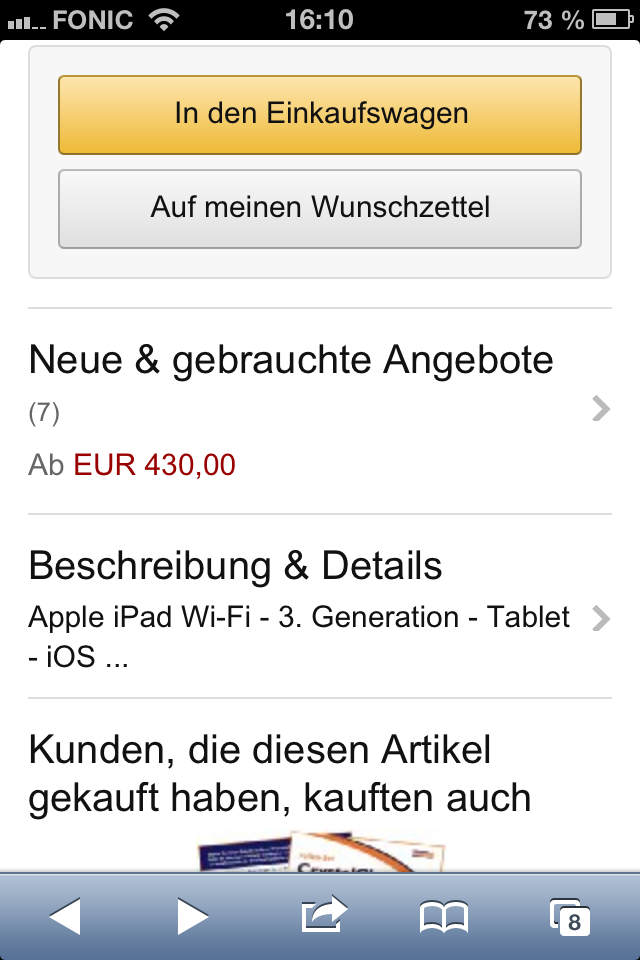
\includegraphics[width=1\textwidth]{img/amazon.png}
		\caption{Mobile Webseite}\label{fig:amazon}
	\end{subfigure}
	\begin{subfigure}[b]{0.6\textwidth}
		\centering
		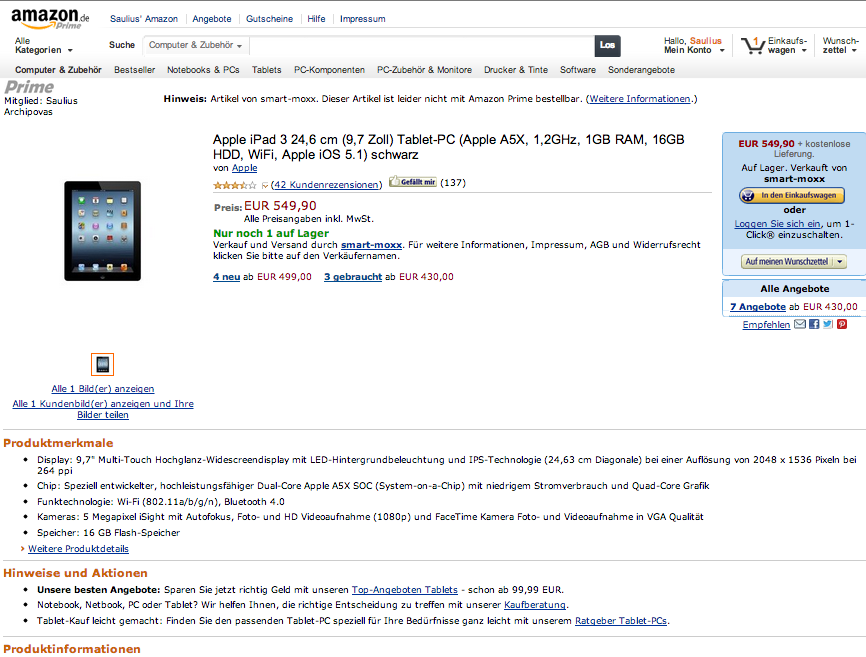
\includegraphics[width=1\textwidth]{img/amazonFull.png}
		\caption{Normale Webseite}\label{fig:amazonFull}
	\end{subfigure}
	\caption{Webseiten von Amazon}\label{fig:amazonSites}
\end{figure}

\subparagraph{Mehr Inhalt, weniger Navigation} 
\label{subp:entferne_das_fett} 

Auch die Konzentration auf den Inhalt und nicht die Navigation sollte in mobilen Kontext bevorzugt werden\cite[Seite 52]{mobileFirst}. So hat der Besucher der Kategorie "Suche" oder "Erforschen/Spielen" vielleicht wenig Zeit um Inhalt zu konsumieren, daher sollte  solcher Benutzer nicht mit eine Sitemap überfordert werden, oder überlegen wo er jetzt hin soll. Als gutes Beispiel dient hier Youtube App, die einen bequemen direkten Einstieg für Konsum ausgelegt ist, da es es schon Videos für den Benutzer vorschlägt (siehe Figure~\ref{fig:youtube}). Die Navigation ist unter einen Bedienknopf unterlegt, und somit spart die Zeit für den Benutzer sowie Platz auf den Bildschirm falls ein schnelles Konsum durch den Benutzer erwünscht ist.

\begin{wrapfigure}{r}{0.5\textwidth}
	\begin{center}
	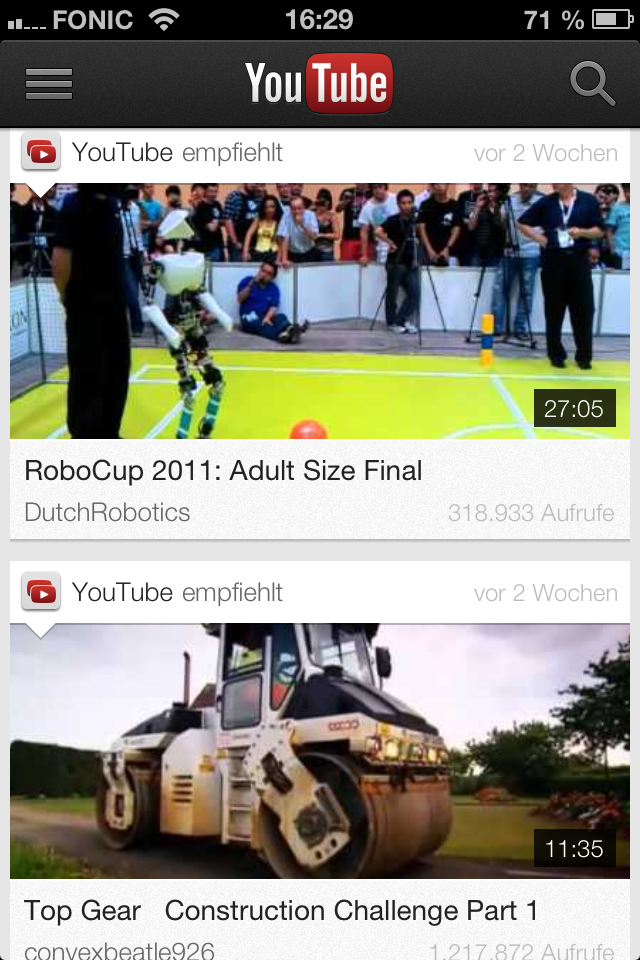
\includegraphics[width=0.3\textwidth]{img/youtube.png}
	\caption{Youtube}\label{fig:youtube}
\end{center}
\end{wrapfigure}

\subparagraph{Schneller Zugriff auf Wichtige informationen} 
\label{subp:subparagraph_name}

Wie im Szenario "Suche", will der Benutzer nicht immer in das Innenleben von Programmen eintauchen, nur um kleine wichtige Bruchteil der Information zu gewinnen. Deshalb sollte man wichtige Informationen schon beim einem Streifblick erkennbar sein(vgl. \cite[Seite 54]{mobileFrontier} und \cite{Neil:2012uf}). Als Beispiel dient hier iPhone Startansicht. Hier sind man die Piktogramme so gestalten, dass sie wichtige Information selbst beinhalten. So beinhaltet etwa die Piktogramm von iOS Kalender den Tag, siehe Beispiel in Bild~\ref{fig:iconIos}. Auch eine die Piktogramme auf können Hinweise leifern, falls neue Informationen existieren, wie bei Errinerungs Piktogram, siehe in Bild~\ref{fig:iconIos}.

\begin{wrapfigure}{r}{0.5\textwidth}
	\begin{center}
	
	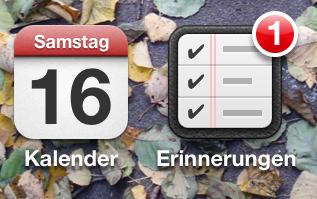
\includegraphics[width=0.3\textwidth]{img/iconIos.png}
	\caption{Schneller Zugriff auf Informationen}\label{fig:iconIos}
\end{center}
\end{wrapfigure}

\subparagraph{Reduziere Kognitive Aufgaben} 
\label{subp:reduziere_kognitive_aufgaben_}

In den mobilen Kontext ist der Benutzer meistens mit verschiedene Aufgaben beschäftigt, so ist auch die Verfügbarkeit der Aufmerksamkeit viel weniger, als etwa in Büro. Bei Gestaltung von Applikationen, mit dennen in mobilen Kontexten gerarbeitet werden soll immer berücksichtigt werden. So soll Anwendungen entstehen, die das unnötige Denken abnimmt. So können die typischen "Wo bin ich" Hinweisen angezeigt werden, oder eine klare Strukturierung der Navigation sowie des Layouts viel helfen. 

Auch die Elementen der Benutzeroberfläche muss den Benutzer nicht überfordern. So sollten unnötige Animationen in eine Anwendung vermieden werden, da sie den Anwender unnötig ablenken oder für längere Zeit unnötig seine Aufmerksamkeit lenken können. Solche Ablenkungen können sogar auch den Benutzer gefähren, da er von seine Tätigkeiten in Realen Welt abbringen und somit sagar zu Unfählen führen können (vgl. \cite{Nasar:2008cc})

\subparagraph{Reduziere Navigationstiefe} 
\label{subp:reduziere_das_w_hlen}

Eine Hierarchisch aufgebaute Navigation ist ein viel benutztes Navigationsmuster in Webseiten sowie Desktop Applikationen. Dieses Muster sollte auch für Applikationen für mobilen Kontexten benutzt weden. Dabei muss beachtet werden dass die Tiefe der Navigations nichts zu groß halten wird. Mit jede weitere Tiefe muss der Benutzer sich mehr Erinnern und Abrufen, was in mobilen Kontext schwierig wird, weil er oft Abgelengk und meistens nur 4 Sekunden Fokus auf die Applikation hat\cite{Oulasvirta:2005vn}. Bei nicht mobilen Kontexten wurde beobachtet, dass solche Navigationen eine Fehleranfälligkeit von 4\% auf 34.0\% bekommt, wenn die Navigationsstruktur von 1 bis 6 erhöht wird (Snowberry at al. Zitiert von \cite{Chae:2004gp}). So sollte eine Goldene Regeln von Hierarchiestufe 3 benutzt werden.


\subparagraph{Nutze alternative Ein- und Ausgabequellen}
\label{subp:nutze_alternative_eingabenger_ten}

Die Interaktion mit den nobilen Gerät kann in einem mobilen Kontext durch vieles beeinflusst werden. So kann der Benutzer etwa beim Fahren einen Autos nicht mit der Hand bedient werden, oder der Blick kann nicht immer auf den Bildschirm ausgerichtet werden. So sollen auch andere Ein- oder Ausgabequellen benutzt werden. Hier bietet sich die Sprache als Ein- und Ausgabemedium.
Auch die Geolokalisierung kann sehr behilflich sein, um etwa Benutzer Informationen anzubieten bei erreichen eines Bestimmten Ortes, ohne Bewusste Eingabe des Ortes durch den Benutzer . Geolokalisierung kann auch Benutzer helfen, weniger Informationen für eine Suche anzugeben, wenn etwa er nach eine Kaffe sucht. So können schon in voraus Kaffes in Unmittelbare nähe gesucht werden.

Die Benutzung von Status-Led oder Vibration kann Benutzer auf Ereignisse Hinweisen, ohne dass er Immer auf den Bildschirm es sehen muss. So kann man in Android Notifications benutzen, um etwa die Status-LED mit bestimmte Farbe und Intervallen blinken zu lassen (vgl. \cite{androidNotApi}). Benachrichtigungen birgen auch viele gefahren, wenn sie nicht durchdacht benutzt werden. So kann es leicht passieren, dass der Benutzer mit Benachrichtigungen regelrecht überflutet wird, und nicht mehr auf erfühlung seine gewünschte aufgaben Konzentrieren kann.  

\subparagraph{Designe für Unterbrechungen und ermögliche eine Fortsetzung}
\label{subp:erm_gliche_eine_fortsetzung}

Im mobilen Kontexten wird der Benutzer oft unterbrochen in seine Aufgaben oder er hat nicht viel Zeit seine Aufgaben zu beenden. So sollen auch eine Anwendung Möglichkeiten bieten die Aufgaben später zu Erledigen. Auch sollten Benutzereingaben oder der Anwendungszustand nicht zurückgesetzt werden nach bestimmten Zeit, um den Benutzer eine Fortsetzung seiner Aufgabe zu ermöglichen.

Was man schon von Webformularen kennt, wenn man zurück geht, und die Formulare über Browser oder mittels Javascript abgespeichert werden können. 
Dabei beiden auch auf mobilen Systemen die Hersteller Apple und Google APIs für Zwischenspeicherung der Information, falls der Benutzer die Applikation kurz schließt.  Daher wird es empfohlen, bei Neustadt der Applikation, den Benutzer von den Letzten Punkt, wo er sich in System befunden hat, seine Arbeit fortzuführen. Zwar wenn der Benutzer dies nicht zu wünschen wollte, kostet ihn dass zurückgehen auf der startweite meistens nur einen klick, statt mehrere eingaben und Navigation fürs erreichen bestimmten alten zustand 

% - In mobilen kontext wird man ständig unterbrochen
% - Ausfühlen von Formularen, 

% Read it later beispiele, mobileFirst seite 27

\subparagraph{Fokussiere auf Erfahrungen, die nur mobil auftreten können} % (fold)
\label{subp:fokussiere_auf_erfahrungen_die_nur_mobil_auftreten_k_nnen}

Es wurde vier Kategorien in diesen Kapitel eingeführt, die den Interaktions... beschreiben. Die mobile Anwendungen sollten auch diese bedienen, und nicht versuchen einen Stationären Arbeitsplatz zu imitieren. Auch die Erfahrungen, die nur mobil auftreten können, sollten berücksichtigt werden. Zum Beispiel bei Eine Notiz Applikationen, man würde den Benutzer ermöglichen Lokalisierungsinformationen oder Schnelle Schnappschüsse zu speichern. 

Ein schönes Beispiel beitete Yahoo sketch a search, die leider nicht mehr Angeboten wird \footnote{http://techcrunch.com/2012/01/30/yahoo-shuts-down-10-mobile-apps-says-its-going-mobile-first/ }, wie in FIGURE. So konnte man den Bereich, in den man eine lokale suche machen wollte mit einen Oval zu beschränken.

% man muss auch den kontent anpassen, an den bedürfniss, seite 72 mobileFirst

\subsection{Gestaltung von Diensten}
\label{sub:gestaltung_von_diensten}

Nicht nur der Visuelle Design von der Applikation muss für mobilen Einsatz angepasst werden, sondern auch die Dienste, die der Applikation anbietet, den mobilen Einsatz unterstützen. Man kann auch die Dienste erweitern, um einen Besonderheiten der Mobilität der benutzer sowie des Geräts auszunutzen.

Wenn man mit einen relativ kleinen mobilen Gerät, wie einem Smartphones unterwegs seine Aufgaben erledigt, will man auch bei wechseln des Gerätes seine Aufgaben fortzuführen. So soll die Anwendungen dies solche Gerätenmobilität anbieten und dabei aktiv ihn unterstützen. Als gutes Beispiel dient hier eine Anwendung für Notizen Evernote. So kann man mit den Mobilen Gerät Notizen oder Photos hochladen, und sie weiter am beliebigen Rechner mit einem Internetanschluß weiter zu bearbeiten oder umgekehrt. Auch der Dienst Photostream von Apple bietet eine Gerätenmobilität und synchronisation: So kann man mit seinen iPhone etwas Fotografieren, und schon nach wenigen Sekunden den Bild am seinem Rechner mit iPhone bearbeiten (Photo??????). 



% - Hier ab seite 90 (mobileFrontier) paar stichpunkte nehmen. Ist aber mehr von presi http://www.slideshare.net/preciousforever/patterns-for-multiscreen-strategies abgeleitet. 

% Themen: Wechsel zwichen Geräten, da man immer im bewegung ist. So sollen Dienste gerätewechsel unterstützen. Auch die aufgaben, die man erledigt, sollten auf anderen gerät oder ort weiterzzführbar sein.

% Dienste sollen auch so angepasst werden, dass die im Kernaufgaben auf beliebigen gerät laufen können.

% Man sollte auch dabei aufpassen, dass man mit eine Symbiose von geräten vorhanden sein sollte. Wie etwa dass man mit einen iPhone einen Fernseher steuern kann. Also anhand des Kontextes und Ortes dienste angeboten werden sollten

% \subparagraph{Dienstkoherenz und Synchronisation}
% \label{subp:diensmobilit_t}

% Beispiel: Evernote

% - Erreichung von diesnten von beliebigen gerät.


% \subparagraph{Gerätemobilität} 
% \label{subp:ger_temobilit_t}

% - Gerätemobilität: Benutzung von diensten in Jeden gerät. 
\subsection{Wearable Computing} 
\label{sub:wearable_computers}

Wearable Computing, oder Tragbare Datenverarbeitung, ist das Forschungsgebiet, das sich mit den der Entwicklung von tragbaren Computersystemen (Wearable Computers) beschäftigt \footnote{citate aus wikipedia }. So wird versucht alltägliche Aktivitäten oder Bedürfnisse des Benutzers  von der Computersysteme zu erleichtern oder sogar ermöglichen, dabei aber tritt der Computersystem im Hintergrund. Die Geräte können beliebige Form annehmen und Funktion erfühlen: von eine Armbanduhr, die ähnlich den Smartphone funktioniert \footnote{http://www.zeit.de/digital/mobil/2013-01/smartwatch-wearable-computer} bis einem  Ring, der die Pulsrate sowie Sauerstoffgehalt in Blut misst \footnote{http://www.sciencephoto.com/media/349431/view}.  Um eine kurze Einführung in Gestaltungsprinzipien im Wearable Computing zu ermöglichen, wird wir auf die Benutzung von Wearable Computing in Arbeitsumfeld und die Forschung die im TZI Wearable Labs begrenzen geschehen und beschränken uns auf die Head-Up-Display Ausgabegeräten.

Wearable Computing kann arbeiten in Industrie (Wartungs-, Lagerarbeit), Gesundheitspflege und anderen Bereichen erleichtern \cite{Witt:2006hi},\cite{Lawo:2008gg}). 



So kann als eine typische Kleidung, die in TZI benutzt wird einen HUD, eine Tragbare Tastatur sowie eine Handschuh mit Steuerungskomponenten hier angesehen werden. Die Ausgabe von den Computern kann mittels eines Displays in einem HUD benutzt werden, und die Eingabe mittels eine Tastatur sowie eine Steureungshandschuh erfühlt werden. Die physikalischen grenzen der Auge, also die Möglichkeit von eine Fokusierungslänge von etwa 20 cm, also ihre Resulation sowie die Mögliche entfernung von HUD Displays, ergeben eine Einschränkung der möglichen visuellen Darstellung von GUI Komponenten auf einen HUD. 

Anders als in stationären Arbeitsumfelder, wo meistens nur eine Hauptaufgabe am einem Rechner bearbeitet wird, es werden in Wearable Computing erwartet, dass der Benutzer zwei Aufgaben erfühlt \cite{Witt:2006hi}. Diese Aufgaben können ins Primäre und Sekundäre Aufgaben eingeteilt werden. Die Primäre Aufgabe besteht meistens aus einer Interaktion mit dem Umwelt, etwa drehen einer Schraube oder Scannen eines Paketes. Primäre Aufgaben können durch Benutzung des tragbaren Computersystemen erleichtert werden, die als sekundären Aufgaben beschrieben werden können. Sekundären Aufgaben wären etwa Bestätigung von einschrauben einer Schraube oder zeigen einer visuelle Information über gerade eingescannten Paket. 

- wichtig ist die ablenkbarkeit in eine arbeit

Um die Aufmerksamkeit des Benutzers zu bekommen, können 4 Benachrichtigungsysteme benutzt werden: "sofortige", "verhandelbare", "vermittelte" und "geplante" \cite{McFarlane:1999um}. Bei der sofortige, wird der benutzer sofort imformiert über neu Information. Solche Benachrichtigungen sind etwa nützlich bei der Betreuung von Auszubildenden in Autowerksädtden durch den Computer eingesetzt werden. So kann anhand eines arbeitsschrits, die benötigte werkzeuge auf den HUD angezeigt werden. Bei der verhandelbare Benachtichtigungsysteme werden die 

Falls eine sekundäre Aufgaben existiert und erledigt werden muss, sollen dabei der Benutzer nicht zu sehr von der Primären aufgaben ablenkt werden. Erstens man muss nachdenken wie er auf der sekundäre Aufgabe aufmerksam gemacht werden muss, zweitens wie soll die Interaktion mit den Computer erfolgen. 





 So kann der Rechner den Benutzer signalisieren, ob er etwa die richtige Schraube genommen hat, oder etwa wo der packet abzulegen sei. Hier sieht man schon die schweirigkeiten, bei der Interaktion zwischen Computersystem und den Benutzer: der Benutzer soll nicht zu viel abgelegt werden von der primäre Aufgabe, weil vieleicht er muss dabei aufpassen, das er die schraube aus den Händen nicht verliert,. Als weiteres muss der System

 Es muss beachtet werden, dass der Benutzer so wenig wie möglich von der primäre Aufgabe abgelenkt wird. Auch der Blickfeld von der Benutzer soll minimal begrenzt werden.


- Mobiles kontext smartphone: sekundäre aufgabe ist der smathphone, dabei ist man in mobilen kontext, den man zwichendurch wechselt. Dabei 
- Hilfe bei HUD displays, so kann man mit einen kurzen blick auf die ausgabe angucken, und dabei Freihandarbeiten



GUI: 
-  Anzeige ist limitiert durch der Resulution von der Auge \cite[Seite 60]{Starner:2001eu}
- die benutzung der Hände für interaktion mit eine Anwendung sollte minimiert werden (vgl. \cite{Rekimoto:gu})
- Hierarchie navigation ist vorteilhaft, da man keine pointer interaktion hat \cite{Blasko:ug}
x- Die 4 Notifikation systeme für kurze ablenkung \cite{McFarlane:1999um}: "Immediate", "negotiated", "mediated", "Scheduled". Keine ist war der klare gewinner, sondern jeder hat seine vorteile und nachteile. In der Studie \cite{Nilsson:cq} wurde der Scheduled hat besser abgeschnitten wie bei der Effizienz sowie auch der subjektiver meinung. Es wird in der studie rezumiert, dass man besser sofort die aufgabe Anzeigt, statt eine Ankündigung anzumelden, da der Wearable Computer in diesenfall aufdriglich ist, und notifications es mehr machen.
- Als alternative wäre eine benutzung der Sprache, wobei laut Lawo et al. \cite{Lawo:2008gg}, war es eines der ineffizienter Methoden. Die Problematik lag an der Software, wo der nicht nur die richtige spracherkennung sondern auch der Akzent der Benutzer zur Problemen führte.

- Eingabe und ausgabegerätem??? DIMA!!!

- Mögliche eingabegeräte \cite{Witt:we}
